\subsection{Which distances to use?}

\textbf{How does the count rate of one detector change with the distance?}\\
The count rate of a detector follows the inverse square law with respect to distance, i.e., it drops by a factor of $d^{-2}$ as the distance $d$ from the detector increases.\\

\textbf{How does the coincidence rate change with the distance? Give a formula!}\\
Since coincidences require both detectors to register radiation, the coincidence rate is related to the distance of both detectors as $f \propto d_1^{-2}d_2^{-2}$.\\

\textbf{How does the asymmetry seen in the experiment differ from the theoretical prediction? Again, give a formula.}\\
The asymmetry in the experiment arises due to the presence of noise, which we can take to be Gaussian in nature. The probability distribution for Gaussian noise is
$$p(x) = \frac{1}{\sqrt{2\pi\sigma^2}}e^{\frac{-x^2}{2\sigma^2}}$$
where $\sigma$ is the variance of the noise.\\

\textbf{How do the correction factors influence the error of the corrected correlation coefficients?}\\
As the correlation coefficients are scaled down by the correction factors, the error in them is also scaled down by this factor.\\

\textbf{Using the values provided in Siegbahn for 2 ”× 2 ” crystals: which distance is likely to yield most precise results?}\\
According to the data in Siegbahn, keeping the detectors $10\,$cm away from the source is most likely to yield precise results. This is simply due to the smaller solid angle the detector takes up by being further away. In an ideal case, the angular correlation measurement would occur at a single point, hence reducing the solid angle improves the values we measure.\\

\subsection{Which angles to pick?}

The theoretical prediction for the angular correlation of 4-2-0 cascade is
$$f(\theta) = N(1 + A_{22}P_2(\cos^2\theta) + A_{44}P_4(\cos^4\theta)).$$
With Legendre polynomials
$$P_2(x)=\frac{1}{2}(3x^2-1)\;\text{and}\;P_4(x)=\frac{1}{8}(35x^4-30x^2+3)$$
this can be written as
$$f(\theta) = A(1 + B\cos^2\theta + C\cos^4\theta)$$
with 
\begin{align}
  A&=N(1+\frac{3}{8}A_{44}-\frac{1}{2}A_{22})\\
B&=\frac{A_{22}\frac{3}{2}-A_{44}\frac{30}{8}}{1+\frac{3}{8}A_{44}-\frac{1}{2}A_{22}}\\
C&=\frac{\frac{35}{8}A_{44}}{1+\frac{3}{8}A_{44}-\frac{1}{2}A_{22}}\\
\end{align}
where $A$ is a scaling factor and $B$ and $C$ are the parameters we're interested in. By changing parameters instead to $\alpha = B+C, \ \beta = B-C$, the above function changes to
$$f(\theta) = A\left(1 + \left( \frac{\alpha+\beta}{2} \right)\cos^2\theta + \left( \frac{\alpha-\beta}{2} \right)\cos^4\theta\right).$$
The function is plotted agains the angle and is shown in \Cref{fig:cds}.
\begin{figure}[H]
	\begin{center}
		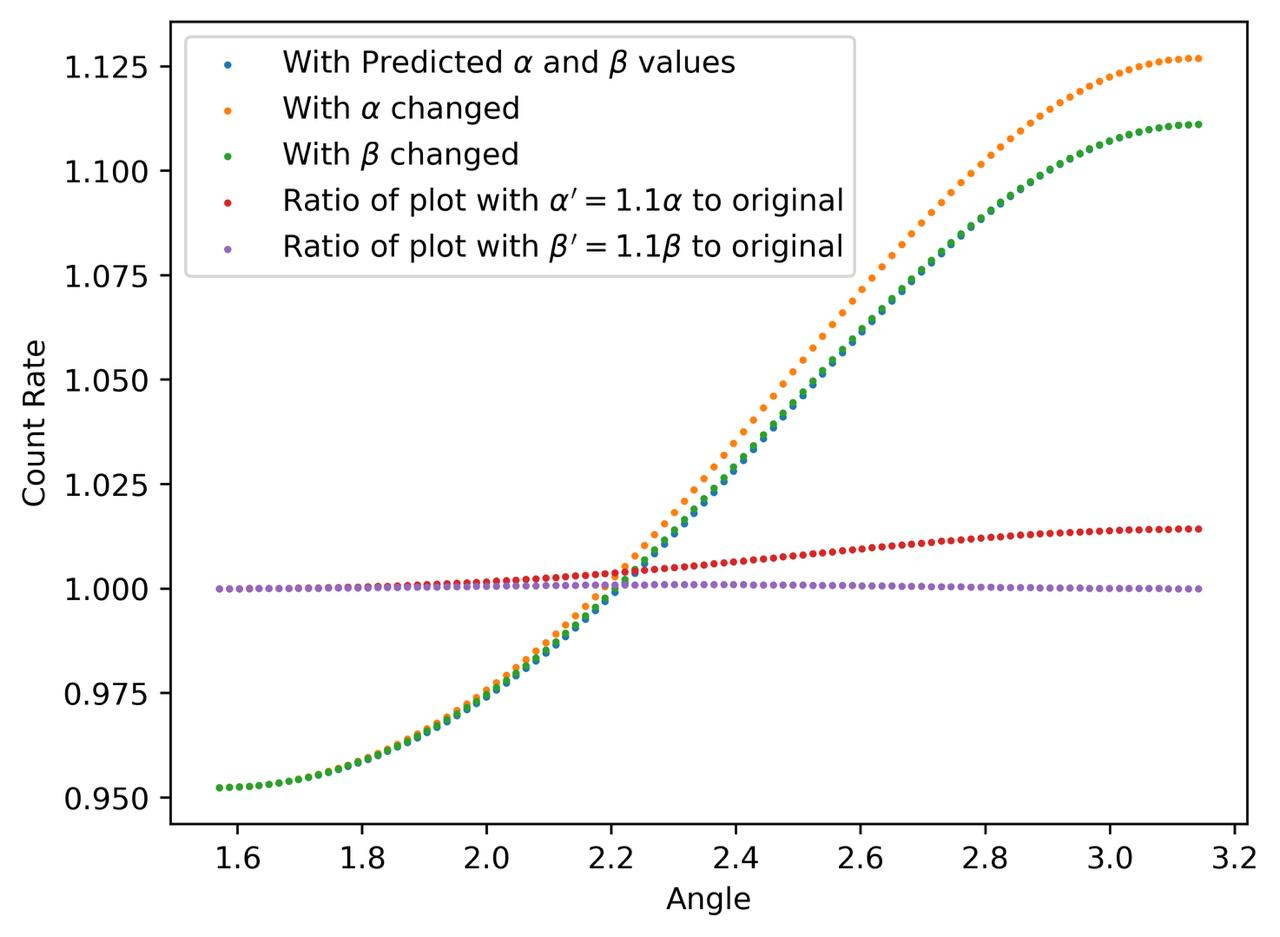
\includegraphics[width=1\textwidth]{../images/angles.jpeg}
	\end{center}
	\caption{Angular Correlation Function and their Variation}\label{fig:cds}
\end{figure}
Here $\alpha$ and $\beta$ are varied by \SI{10}{\%}. The ratios of varied and original values is also plotted to see the major differences. Change in $\alpha$ has here the most impact, whereas $\beta$ has close to no influence on the function. It is seen that around $\SI{180}{\degree}$ the function experiences the most change. Therefore the measured angles should range from approximately $\SI{120}{\degree}$ to $\SI{240}{\degree}$. Here the constants $A_{22}=\SI{0.102}{}$ and $A_{44}=\SI{0.0091}{}$ are chosen since the $4-2-0$ cascade is expected. Since at the end of the expereiment also other cascades are compared to the measurements, the measured angle range is still chosen to be from $\SI{90}{\degree}$ to $\SI{270}{\degree}$ in $\SI{15}{\degree}$ steps, totaling to 13 angles.


\subsection{How to correct for de-adjustment?}

Let the source be at distance of $k$ away from the centre of the circle in the direction of the stationary detector. We can determine the new distance between the source and the moving director at an angle $\theta$ using the Law of Cosines (where $\theta$ is the angle between the lines formed by joining the centre of the circle to the two detectors). If the original distance, the radius of the circle was $r$, the new distance is
$$d = \sqrt{r^2 + k^2 - 2rk\cos\theta}$$.
Since for a circle of radius 1, the count rate would be $f(\theta) = 1$, and since the count rate follows the inverse square law with distance from the source, we know the count rate originally was
$$f(\theta) = \frac{1}{r^2}$$
which becomes now
$$f(\theta) = \frac{1}{d^2} = \frac{1}{r^2 + k^2 - 2rk\cos\theta}$$
This will appear in the data as a high spike near $\theta=0\degree$ before sharply falling and plateauing towards 0 at $\theta=180\degree$. The larger the deviation from the centre, the sharper the fall and the closer the latter part of the data will be to 0.\\
